\documentclass{beamer}

\usepackage[T2A]{fontenc}
\usepackage[utf8]{inputenc}
\usepackage[russian]{babel}
\usepackage{graphicx}
\usepackage{todonotes}
\usepackage{listings}
\usepackage{adjustbox}

\usetheme{Madrid}
\usecolortheme{whale}

\hypersetup {
    unicode = true
}

\title[]{Инструментальная среда для анализа программных систем}
\author[А.М. Полоцев]{
    А.М. Полоцев, гр. 63501/13\\
    научный руководитель: к.т.н. доцент В.М. Ицыксон
}
\institute[]{Санкт-Петербургский Политехнический Университет}
\date[XLII Неделя науки]{XLII Неделя науки}

\begin{document}
%===============================================================================
\frame{\titlepage}
%===============================================================================
%===============================================================================
\begin{frame}
\frametitle{Постановка задачи}

\begin{itemize}
    \item В различных методах анализа часто решаются похожие задачи:
    \begin{itemize}
        \item Построение моделей программы (AST, CFG и т.п.)
        \item Построение метрик
        \item Реинжиниринг программного обеспечения (оптимизация, рефакторинг и т.п.)
        \item Визуализация свойств системы
    \end{itemize}
\end{itemize}
\pause
\begin{alertblock}{}
    \center{Обычно эти задачи решаются вручную}
\end{alertblock}

\end{frame}
%===============================================================================
%===============================================================================
\begin{frame}
\frametitle{Разработка инструментального средства}

\begin{itemize}
    \item Цели
        \begin{itemize}
            \item Автоматизация анализа
            \item Визуализация свойств системы
        \end{itemize}
    \item Требования
        \begin{itemize}
            \item Поддержка анализа объектно-ориентированных языков
            \item Извлечение различных моделей анализируемой системы
            \item Встроенные средства отображения
            \item Модульная расширяемая структура
            \item Экспорт разных артефактов системы во внешние отчеты
            \item Предоставление API к разработанным методам анализа
        \end{itemize}
\end{itemize}
\end{frame}
%===============================================================================
%===============================================================================
\begin{frame}
\frametitle{Архитектура инструментального средства}

\begin{figure}[h!]
    \begin{center}
        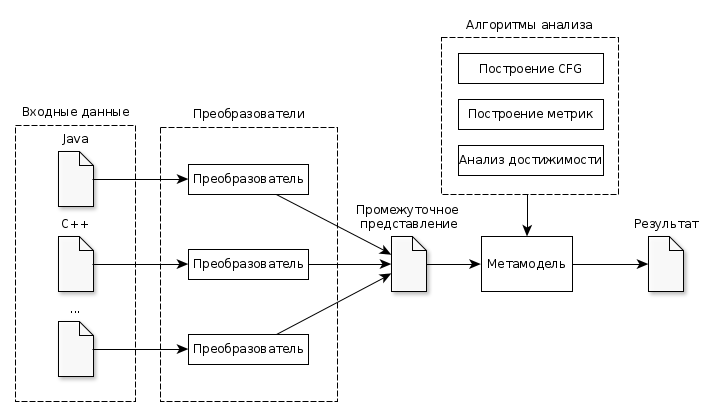
\includegraphics[width=\textwidth]{img/architecture.png}
    \end{center}
\end{figure}
\end{frame}
%===============================================================================
%===============================================================================
\begin{frame}
\frametitle{Разработка метамодели}

\begin{itemize}
    \item Цели:
        \begin{itemize}
            \item Унификация представления системы для проведения анализа и трансформаций
        \end{itemize}
    \item Требования:
        \begin{itemize}
            \item Независимость от языка описания анализируемой системы
            \item Достаточная мощность для извлечения различных моделей
            \item Расширяемость путем добавления новых метаданных
        \end{itemize}
\end{itemize}

\end{frame}
%===============================================================================
%===============================================================================
\begin{frame}
\frametitle{Разработка метамодели. MOF}

\begin{itemize}
    \item Meta Object Facility (MOF)
    \item Стандарт, разработанный Object Management Group (OMG)
    \item Метаметамодель для описания метамоделей
    \item Поддержка объектно-ориентированной парадигмы
    \item Четырехуровневая архитектура
    \begin{itemize}
        \item Уровень метаметамодели (M3)
        \item Уровень метамоделей (M2)
        \item Уровень моделей (M1)
        \item Информационный уровень(M0)
    \end{itemize}
\end{itemize}

\end{frame}
%===============================================================================
%===============================================================================
\begin{frame}
\frametitle{Разработка метамодели. MOF}

\begin{figure}[h!]
    \begin{center}
        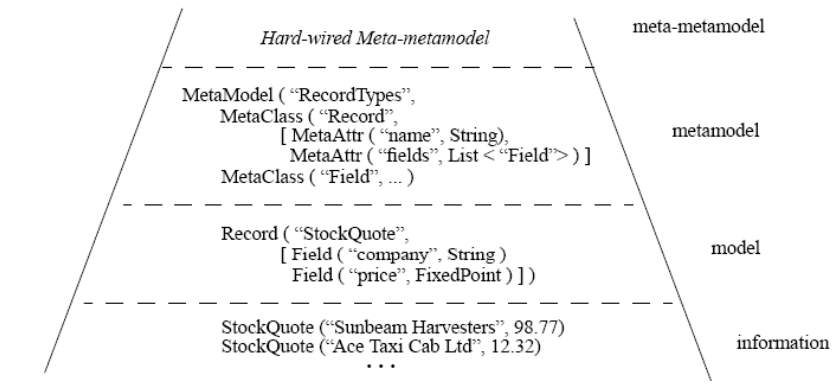
\includegraphics[width=\textwidth]{img/metadata_architecture}
    \end{center}
\end{figure}

\end{frame}
%===============================================================================
%===============================================================================
\begin{frame}
\frametitle{Разработка метамодели. Диаграмма классов}

\begin{figure}[h!]
    \begin{center}
        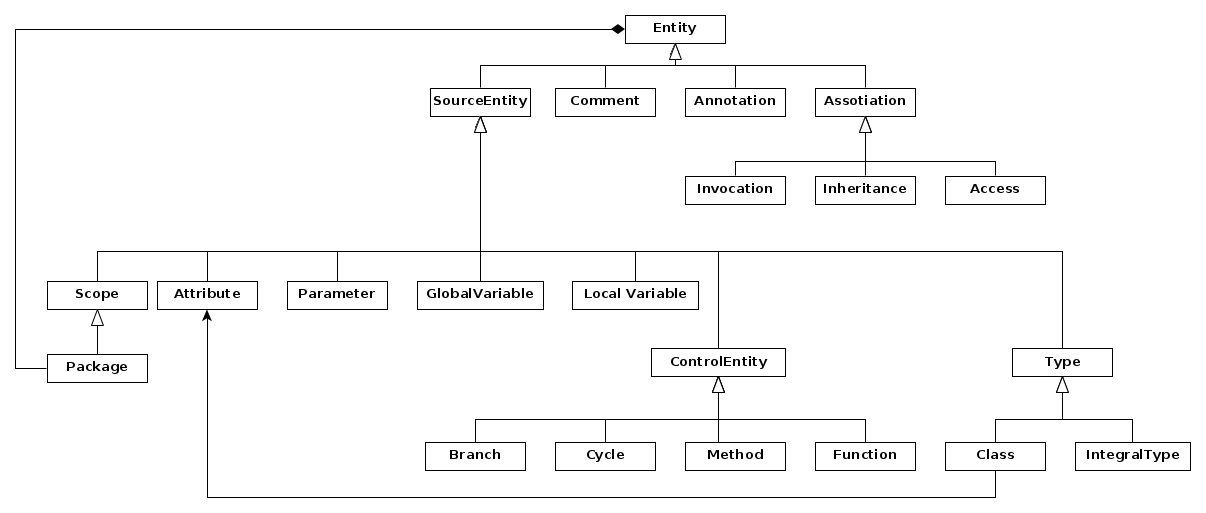
\includegraphics[width=\textwidth]{img/metamodel.png}
    \end{center}
\end{figure}

\end{frame}
%===============================================================================
%===============================================================================
\begin{frame}
\frametitle{Преобразование исходного кода в метамодель}

\begin{itemize}
    \item Для каждого языка программирования необходимо написать специализированные
    преобразователи
    \item Задачи преобразователей - генерация промежуточного представления
    \item Для написания преобразователей предполагается разработать библиотеку для
    генерации промежуточного представления
\end{itemize}

\begin{figure}[h!]
    \begin{center}
        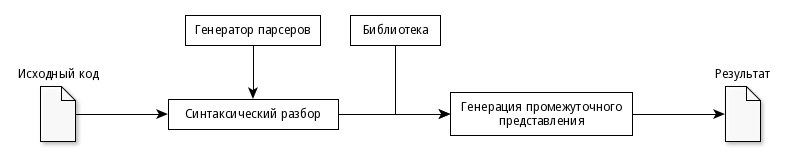
\includegraphics[width=\textwidth]{img/parser_architecture.png}
    \end{center}
\end{figure}

\end{frame}
%===============================================================================
%===============================================================================
\begin{frame}
\frametitle{Выбор промежуточного представления}

\begin{itemize}
    \item Требования:
    \begin{itemize}
        \item Полнота описания
        \item Расширяемость
    \end{itemize}
    \item Формат XMI (XML Metadata Interchange):
    \begin{itemize}
        \item Разработан OMG
        \item Основан на XML
        \item Предназначен для сериализации метаданных
    \end{itemize}
\end{itemize}

\end{frame}
%===============================================================================
%===============================================================================
\begin{frame}[fragile]
\frametitle{Выбор промежуточного представления. Пример.}

\begin{columns}
    \begin{column}[c]{0.2\textwidth}
        \begin{figure}[h!]
            \begin{center}
                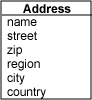
\includegraphics[width=0.8\textwidth]{img/xmi_example.png}
            \end{center}
        \end{figure}
    \end{column}
    \begin{column}[c]{0.8\textwidth}
        \begin{adjustbox}{width=0.8\textwidth,keepaspectratio}
        \begin{lstlisting}
        <?xml version="1.0"?>
        <XMI xmi.version="1.2" xmlns:UML="org.omg/UML/1.4">
         <XMI.header>
          <XMI.documentation>
           <XMI.exporter>ananas.org stylesheet</XMI.exporter>
          </XMI.documentation>
          <XMI.metamodel xmi.name="UML" xmi.version="1.4"/>
         </XMI.header>
         <XMI.content>
          <UML:Model xmi.id="M.1" name="address" visibility="public"
                      isSpecification="false" isRoot="false"
                      isLeaf="false" isAbstract="false">
           <UML:Namespace.ownedElement>
            <UML:Class xmi.id="C.1" name="address" visibility="public"
                       isSpecification="false" namespace="M.1" isRoot="true"
                       isLeaf="true" isAbstract="false" isActive="false">
             <UML:Classifier.feature>
              <UML:Attribute xmi.id="A.1" name="name" visibility="private"
                             isSpecification="false" ownerScope="instance"/>
              <UML:Attribute xmi.id="A.2" name="street" visibility="private"
                             isSpecification="false" ownerScope="instance"/>
              <UML:Attribute xmi.id="A.3" name="zip" visibility="private"
                             isSpecification="false" ownerScope="instance"/>
              <UML:Attribute xmi.id="A.4" name="region" visibility="private"
                             isSpecification="false" ownerScope="instance"/>
              <UML:Attribute xmi.id="A.5" name="city" visibility="private"
                             isSpecification="false" ownerScope="instance"/>
              <UML:Attribute xmi.id="A.6" name="country" visibility="private"
                             isSpecification="false" ownerScope="instance"/>
             </UML:Classifier.feature>
            </UML:Class>
           </UML:Namespace.ownedElement>
          </UML:Model>
         </XMI.content>
        </XMI>
        \end{lstlisting}
        \end{adjustbox}
    \end{column}
\end{columns}

\end{frame}
%===============================================================================
%===============================================================================
\begin{frame}
\frametitle{Направления дальнейшей разработки}

\begin{itemize}
    \item Реализация преобразователя для языка Java
    \item Разработка методов трансформации метамодели
    \item Разработка графического интерфейса
    \item Разработка библиотеки моделей
\end{itemize}

\end{frame}
%===============================================================================
%===============================================================================
\begin{frame}
\frametitle{Результаты}

\begin{itemize}
    \item Сформулированы задачи анализа, требующие автоматизации
    \item Разработана архитектура инструментального средства
    \item Разработана метамодель
    \item Предложен формат промежуточного представления для экспорта метамодели
\end{itemize}

\end{frame}
%===============================================================================
%===============================================================================
\begin{frame}
\frametitle{Спасибо за внимание}
\center{\resizebox{60pt}{80pt}{?}}
\end{frame}
%===============================================================================
\end{document}
